\usepackage{wasysym}%%%%%%%%%%%%%%%%%%%%%%%%%%%%%%%%% LAB-5 %%%%%%%%%%%%%%%%%%%%%%%%%%%%%%%%%%
%>>>>>>>>>>>>>>>>>>>>>>>>>> ПЕРЕМЕННЫЕ >>>>>>>>>>>>>>>>>>>>>>>>>>>>>>>>>>>

%>>>>> Информация о кафедре
%\newcommand{\year}{2021 г.}  % Год устанавливается автоматически
\newcommand{\city}{Санкт-Петербург}  %  Футер, нижний колонтитул на титульном листе
\newcommand{\university}{Национальный исследовательский университет ИТМО}  % первая строка
\newcommand{\department}{Факультет программной инженерии и компьютерной техники}  % Вторая строка
\newcommand{\major}{Направление программная инженерия}  % Треьтя строка
% Пусть будет. Проще закоментить лишнее.
\newcommand{\education}{Образовательная программа системное и прикладное программное обеспечение}  % четвертая строка
%\newcommand{\specialization}{}  % пятая строка

%<<<<< Информация о кафедре
%Ашч
%>>>>> Назание работы
\newcommand{\reporttype}{ОТЧЕТ ПО ЛАБОРАТОРНОЙ РАБОТЕ} % тип работы, (главный заголовок титульного листа)
\newcommand{\lab}{Лабораторная работа}          % вид работы
\newcommand{\labnumber}{№ 2}                    % порядковый номер работы
\newcommand{\subject}{Программирование}         % учебный предмет
\newcommand{\labtheme}{Принципы ООП}            % Тема лабораторной работы
\newcommand{\variant}{№ 68118}                % номер варианта работы
\newcommand{\student}{Мухамедьяров Артур Альбертович}    % определение ФИО студента
\newcommand{\studygroup}{P3109}                 % определение учебной группы
\newcommand{\teacher}{% принимающий
    Гаврилов А. В.,\\[1mm]% ФИО лектора
    Мустафаева А. В.% ФИО практика
}
%<<<<<<<<<<<<<<<<<<<<<<<<<< ПЕРЕМЕННЫЕ <<<<<<<<<<<<<<<<<<<<<<<<<<<<<<<<<<<


%>>>>>>>>>>>>>>>>>>>>>> ПРЕАМБУЛА >>>>>>>>>>>>>>>>>>>>>>>>>
%>>>>>>>>>>>>>>>>>> ПРЕАМБУЛА >>>>>>>>>>>>>>>>>>>>
\documentclass[14pt,final,oneside]{extreport}% класс документа, характеристики
%>>>>> Разметка документа
\usepackage[a4paper, mag=1000, left=3cm, right=1.5cm, top=2cm, bottom=2cm, headsep=0.7cm, footskip=1cm]{geometry} % По ГОСТу: left>=3cm, right=1cm, top=2cm, bottom=2cm,
\linespread{1} % межстройчный интервал по ГОСТу := 1.5
%<<<<< Разметка документа

%>>>>> babel c языковым пакетом НЕ должны быть первым импортируемым пакетом
\usepackage[utf8]{inputenc}
\usepackage[T1,T2A]{fontenc}
\usepackage[russian]{babel}
% \usepackage{lmodern}
%<<<<<

%\usepackage{cmap} %поиск в pdf

%>>>...>> прочие полезные пакеты
\usepackage{amsmath,amsthm,amssymb}
\usepackage{mathtext}
\usepackage{braket}
\usepackage{indentfirst}
\usepackage{graphicx}
\usepackage{float}
\usepackage{changepage}
\graphicspath{{/home/ivan/itmo/informatics/latex}}
\DeclareGraphicsExtensions{.pdf,.png,.jpg}
%\usepackage{bookmark}

\usepackage[dvipsnames]{xcolor}
\usepackage{hyperref}  % Использование ссылок
\hypersetup{%  % Настройка разметки ссылок
    colorlinks=true,
    linkcolor=blue,
    filecolor=magenta,
    urlcolor=magenta,
%pdftitle={Overleaf Example},
%pdfpagemode=FullScreen,
}

\usepackage{diagbox}
\usepackage[letterspace=150]{microtype} % Спэйсинг (межбуквенный интервал для саголовка) \lsstyle
% \usepackage{csvsimple} %импорт содержимого таблицы из csv

%>>> верстка в 2 колонки
\usepackage{multicol} % многоколоночная верстка
\setlength{\columnsep}{.15\textwidth} % определение ширины разделителя между колонками

\usepackage{tikz} % пакет для векторной графики, чтобы рисовать красивый разделитель колонок
% %> кастомный разделитель колонок
% \usetikzlibrary{arrows.meta,decorations.pathmorphing,backgrounds,positioning,fit,petri}
% \usepackage{multicolrule} % Для кастомизации разделителя колонок
% \SetMCRule{                     % кастомизация разделителя колонок multicolrule
%     width=2pt,
%     custom-line={               % Tikz код для кастомизации линии разделителя
%         \draw [                 % Рисовать
%             decorate,           % декорированную (требуются спец настройки пакетов tikz (см. импорт выше)
%             decoration={        % вид декорирования
%                 snake, % Тип - змейка (волнистая)
%                 amplitude=.5mm, % ширина волн
%                 pre length=0mm, % участок прямой линии от начала
%                 %segment length=0mm, % учасок волнистой линии
%                 post length=0mm % участок прямой линии от конца
%             },
%             line width=1pt,
%             step=10pt
%         ] 
%         (TOP) to (BOT); % сверху и до низа колонки
%     }, 
%     extend-top=-5pt, % Вылезти за верхнюю границу колонки 
%     extend-bot=-7pt % Вылезти за нижнюю границу колонки  
% }
%% < кастомный разделитель колонок
%%<<< верстка в 2 колонки

%>>>>> Использование листингов
\usepackage{listings}
\usepackage{caption}
\DeclareCaptionFont{white}{\color{white}}
\DeclareCaptionFormat{listing}{\colorbox{gray}{\parbox{\textwidth}{#1#2#3}}}

\captionsetup[lstlisting]{format=listing,labelfont=white,textfont=white} % Настройка вида описаний
\lstset{  % Настройки вида листинга
    inputencoding=utf8, extendedchars=\true, keepspaces = true, % поддержка кириллицы и пробелов в комментариях
    language={},            % выбор языка для подсветки (здесь это Pascal)
    basicstyle=\small\sffamily, % размер и начертание шрифта для подсветки кода
    numbers=left,               % где поставить нумерацию строк (слева\справа)
    numberstyle=\tiny,          % размер шрифта для номеров строк
    stepnumber=1,               % размер шага между двумя номерами строк
    numbersep=5pt,              % как далеко отстоят номера строк от подсвечиваемого кода
    backgroundcolor=\color{white}, % цвет фона подсветки - используем \usepackage{color}
    showspaces=false,           % показывать или нет пробелы специальными отступами
    showstringspaces=false,     % показывать илигнет пробелы в строках
    showtabs=false,             % показывать или нет табуляцию в строках
    frame=single,               % рисовать рамку вокруг кода
    tabsize=2,                  % размер табуляции по умолчанию равен 2 пробелам
    captionpos=t,               % позиция заголовка вверху [t] или внизу [b]
    breaklines=true,            % автоматически переносить строки (да\нет)
    breakatwhitespace=false,    % переносить строки только если есть пробел
    escapeinside={\%*}{*)}      % если нужно добавить комментарии в коде
}

\definecolor{codegreen}{rgb}{0,0.6,0}
\definecolor{codegray}{rgb}{0.5,0.5,0.5}
\definecolor{codepurple}{rgb}{0.58,0,0.82}
\definecolor{backcolour}{rgb}{0.95,0.95,0.92}

\lstdefinestyle{mystyle}{
backgroundcolor=\color{backcolour},
commentstyle=\color{codegreen},
keywordstyle=\color{magenta},
numberstyle=\tiny\color{codegray},
stringstyle=\color{codepurple},
basicstyle=\ttfamily\footnotesize,
breakatwhitespace=false,
breaklines=true,
captionpos=b,
keepspaces=true,
numbers=left,
numbersep=5pt,
showspaces=false,
showstringspaces=false,
showtabs=false,
tabsize=2
}
\lstset{style=mystyle}
%<<<<< Использование листингов


\sloppy % Решение проблем с переносами (с. 119 книга Львовского)
\emergencystretch=25pt


%>>>>>>>>>>>>>>>> ДОПОЛНИТЕЛЬНЫЕ КОМАНДЫ {Для соответствия ГОСТ} >>>>>>>>>>>>>>
%>>>>>> математические функции для удобства
\newcommand{\tx}{\text}
\newcommand{\eps}{\varepsilon}
\renewcommand{\phi}{\varphi}
\newcommand{\limit}{\displaystyle\lim}
\newcommand{\oo}{\infty}
\newcommand{\De}{\Delta}
\newcommand{\cd}{\cdot}
\newcommand{\df}{\partial}
\newcommand{\ndash}{\textendash}
\newcommand{\mdash}{\textemdash}

%>>>>> Аннотирование
\newcommand{\note}[2]{\overbrace{#1}^{#2}}% скобка сверху для комментария
% \overset{}{}% для указания символа над другим смиволом
% \underset{}{}% для указания символа под другим смиволом
%<<<<< Аннотирование

%>>>>>> Матрицы
\DeclareMathOperator{\rank}{rank}
\newcommand{\tvec}[1]{\mathbfit{#1}}% "text vector"
\newcommand{\mtx}[1]{\mathrm{#1}}
\newcommand{\transposed}[1]{{#1}^{\mathrm{T}}}
%>>>>>> Матрицы

%>>>>> Скобки
\newcommand{\lt}{\left}
\newcommand{\rt}{\right}
\newcommand{\la}{\langle}% '<'
\newcommand{\ra}{\rangle}% '>'
\newcommand{\avg}[1]{\langle{#1}\rangle}% '<X>'
%<<<<< Скобки

%>>>>> Дроби
\newcommand{\cf}[2]{\cfrac{#1}{#2}}
\newcommand{\fr}[2]{\frac{#1}{#2}}
%<<<<< Дроби


%>>>>> Стрелки
\newcommand{\Rarr}{\Rightarrow}% ⇒ следствие | лучше использовать \implies
\newcommand{\LRarr}{\Leftrightarrow}% равносильно | лучше  использовать \iff
\newcommand{\rarr}{\xrightarrow{}}% → стрелка вправо
\newcommand{\nwarr}{\nwarrow}% ↖ север-запад стрелка
\newcommand{\nearr}{\nearrow}% ↗ север-восток стрелка
\newcommand{\swarr}{\swarrow}% ↙ юг-запад стрелка
\newcommand{\searr}{\searrow}% ↘ юг-восток стрелка

\newcommand{\raises}{\nwarrow}% возрастает
\newcommand{\increases}{\nwarrow}% возрастает
\newcommand{\falls}{\swarrow}% убывает
\newcommand{\decreases}{\swarrow}% убывает

%{{{
\makeatletter
\newcommand{\impliesby}[2][]{\ext@arrow 0359\Leftrightarrowfill@{#1}{#2}}% следствие с надписью
\makeatother
%}}}

%{{{
\makeatletter
\newcommand{\iffby}[2][]{\ext@arrow 0359\Rightarrowfill@{#1}{#2}}% равносильность с надписью
\makeatother
%}}}
%<<<<< Стрелки

% Функции для удобного описания формул: https://tex.stackexchange.com/questions/95838/how-to-write-a-perfect-equation-parameters-description


%<<<<<< математические функции для удобства
%>>>>>> Стиль текста
\newcommand{\hex}[1]{\texttt{0{\footnotesize{x}}#1}}
\newcommand{\ttt}[1]{\texttt{#1}}
%<<<<<< Стиль текста

\newcommand\Chapter[3]{%
% Принимает 3 аргумента - название главы и дополнительный заголовок и множитель ширины загловка (можно ничего)
\refstepcounter{chapter}%
\chapter*{%
%\hfill % заполнение отступом пространства до заголовка
\begin{minipage}{#3\textwidth} % Можно изменить ширину министраницы (заголовка)
\flushleft % Выранивание заголовка по левому краю параграфа (заголовка)
%\flushright % Выранивание заголовка по правому краю параграфа (заголовка)
\begin{huge}%
% Отключена нумерация глав в тексте:
% \textbf{\chaptername\ \arabic{chapter}\\}
\textbf{#1}% Первый заголовок
\end{huge}%
\\% Перенос сторки
\begin{Huge}
#2% Второй заголовок
\end{Huge}
\end{minipage}
}%
% Отключена нумерация для chapter в toc (table of contents), т.е. Оглавлении (Содержании):
% \addcontentsline{toc}{chapter}{\arabic{chapter}. #1}
% Представление главы в содержании:
\addcontentsline{toc}{chapter}{#1. #2}%
}

\newcommand\Section[1]{
% Принимает 1 аргумент - название секции
\refstepcounter{section}
\section*{%
\raggedright
% Отключена дополнительная нумерация chapter в section в тексте документа:
% \arabic{chapter}.\arabic{section}. #1}
% Отключена любая нумарация section в тексте документа:
\arabic{section}. #1%
}

% Отключена дополнительная нумерация chapter в section в toc (table of contents) Оглавлении (Содержании):
% \addcontentsline{toc}{section}{\arabic{chapter}.\arabic{section}. #1}
\addcontentsline{toc}{section}{\arabic{section}. #1}
}


\newcommand\Subsection[1]{
% Принимает 1 аргумент - название подсекции
\refstepcounter{subsection}
\subsection*{%
\raggedright%
% Отключена дополнительная нумерация chapter в section в тексте документа (можно добавить отступ с помощью \hspace*{12pt}):
% \arabic{chapter}.\arabic{section}.\arabic{subsection}. #1}
\arabic{section}. \arabic{subsection}. #1
}
% Отключена дополнительная нумерация chapter в section в Оглавлении (Содержании):
%\addcontentsline{toc}{subsection}{\arabic{chapter}.\arabic{section}.\arabic{subsection}. #1}
\addcontentsline{toc}{subsection}{\arabic{subsection}. #1}
}


\newcommand\Figure[4]{
% Принимает 4 аргумента - название файла изображения, ее размер в тексте, описание, лэйбл (псевдоним в формате "fig:name")
%
\refstepcounter{figure}
\begin{figure}[H] %- \usepackage {float} %[h]
\begin{center}
\fbox{
\includegraphics[width=#2]{#1}
}
\end{center}
\begin{center}
Рис.~\arabic{figure}. #3.
\end{center}
%\caption{#3}
\label{fig:#4}
\end{figure}
}


\newcommand\Table[3]{
% Принимает 3 аргумента --- лэйбл name(#1) (псевдоним в формате "tab:name"), ее описание(#2), содержание таблицы(#3)
% ВАЖНО!: от этого способа страдает нумерация описаний, можно использовать создание таблиц через googlesheet
%
\renewcommand{\arraystretch}{1.2} % Установка высоты строки таблицы по умолчанию, увеличенное на 0.2 пункта
% \refstepcounter{table}% увеличение счетчика таблиц
\begin{table}[Htpb]% "right Here", "top", "new page", "bottom"
\label{tab:#1}% лэйбл таблицы, для ссылок
\resizebox{\columnwidth}{!}{% сжимает очень широкие таблицы, чтобы вместить на страницу
#3% Содержимое таблицы
}
%
\caption{#2}% Описание стандартными средствами для используемого окружения (table)
% \captionof{table}{#2}% Описание стандартными средствами
% \captionof*{figure}{\flushleft \textsc\textbf{Рис. 1.}}% Описание стандартными средствами, как рисунка
%
%%> кастомное описание
% \begin{flushleft}% Кастомное описание
%     % \textsf{%
%         \textbf{%
%             \\[2mm]
%             #2% Описание к картинке
%         }%
%         % \\[8mm]% Отступ
%     % }%
% \end{flushleft}
%%< кастомное описание
\end{table}
\renewcommand{\arraystretch}{1} % возврат установка высоты строки таблицы по умолчанию на 1
}


\newcommand\CustomFigure[4]{ % multicols не умеют в table и figure, поэтому приходится извращаться % вставка таблицы с меткой рисунка
% Принимает 4 аргумента - название файла изображения, ее размер в тексте, описание, лэйбл (псевдоним в формате "fig:name")
%
\refstepcounter{figure}
\begin{figure}[ht]% "here", "top"
\begin{center}
\includegraphics[width=#2]{#1}
\end{center}
%
%\caption{#3}
\captionof{figure}{#3}% описание стандартными средствами
% \begin{center}
\begin{flushleft} % Кастомное описание
\textbf{%
#3% Текст описания
}
\end{flushleft}
% \end{center}
%
\label{fig:#4}% Лэйбл, для ссылок
\end{figure}
}


\newcommand\CustomTableFigure[3]{% multicols не умеют в table и figure, поэтому приходится извращаться % вставка таблицы с меткой рисунка
%
% Принимает 3 аргумента --- лэйбл name(#1) (псевдоним в формате "tab:name"), ее описание(#2), содержание таблицы(#3)
%
\begin{center}
\refstepcounter{figure}
\label{tab:#1}% лэйбл таблицы, для ссылок
\resizebox{\columnwidth}{!}{% сжимает очень широкие таблицы, чтобы вместить на страницу
#3% Содержание таблицы
}
%
\captionof{figure}{#2}% Описание стандартными средствами
% \captionof*{figure}{\flushleft \textsc\textbf{Рис. 1.}}% Описание стандартными средствами
%
\begin{flushleft}% Кастомное описание
% \textsf{%
\textbf{%
\\[2mm]
#2% Описание к картинке
}%
% \\[8mm]% Отступ
% }%
\end{flushleft}
\end{center}
}


\newcommand{\InkscapeFigure}[4]{% Вставки иллюстраций из Inkscape (pdf+latex)
%
% Принимает 4 параметра: #1 название файла, #2 описание, #3 лейбл #4 размер
%
% \begin{minipage}{#4}
\begin{figure}[htbp]
\centering
\def\svgwidth{#4}
\import{./figures/}{#1.pdf_tex}
\caption{#2}
\label{fig:#3}
\end{figure}
% \end{minipage}
}


\newcommand\Equation[3]{% Кастомное оформление выражений
%
% Принимает 3 аргумента --- лэйбл name (#1) (псевдоним в формате "tab:name"), его описание(#2), содержание выражения (#3)
%
\textbf{#2}% описание
\begin{equation}
#3% содержимое выражений
\label{eq:#1}% лэйбл
\end{equation}
}

%<<<<<<<<<<<<<<<<<<<<<<<<<<<< ДОПОЛНИТЕЛЬНЫЕ КОМАНДЫ <<<<<<<<<<<<<<<<<<<<<<<<<<
%<<<<<<<<<<<<<<<<<<<<<< ПРЕАМБУЛА <<<<<<<<<<<<<<<<<<<<<<<<<


%%%%%%%%%%%%%%%%%%% СОДЕРЖИМОЕ ОТЧЕТА %%%%%%%%%%%%%%%%%%%%%
%>>>>>>>>>>>>>>> ''''''''''''''''''''''' >>>>>>>>>>>>>>>>>>
\begin{document}


%>>>>>>>>>>>>>>>> ОПРЕДЕЛЕНИЕ НАЗВАНИЙ >>>>>>>>>>>>>>>>>>>>
% Переоформление некоторых стандартных названий
%\renewcommand{\chaptername}{Лабораторная работа}
    \renewcommand{\chaptername}{\lab\ \labnumber} % переименование глав
    \renewcommand{\contentsname}{Содержание} % переименование оглавления
%<<<<<<<<<<<<<<<< ОПРЕДЕЛЕНИЕ НАЗВАНИЙ <<<<<<<<<<<<<<<<<<<<
% \setlength{\itemsep}{0pt} % установка расстояния между строчками в списках можно использовать локально внутри списка списке
% \setlength{\parskip}{0pt} % 
% \setlength{\parsep}{0pt}  % 

%>>>>>>>>>>>>>>>>> ТИТУЛЬНАЯ СТРАНИЦА >>>>>>>>>>>>>>>>>>>>>
    %>>>>>>>>>>>>>>>>>>> ТИТУЛЬНЫЙ ЛИСТ >>>>>>>>>>>>>>>>>>>>>>>
\begin{titlepage}

    % Название университета
    \begin{center}
        \textsc{%
            \university\\[5mm]
            \department\\[2mm]
            \major\\
            \education\\
%        \specialization\\
        }

        \vfill
        % Название работы
        \textbf{\reporttype\ \labnumber\\[3mm]
        курса <<\subject>> \\[6mm]
        по теме: <<\labtheme>>\\[3mm]
        Вариант \variant\\[20mm]
        }
    \end{center}


    \vfill
    \hfill
% Информация об авторе работы и проверяющем
    \begin{minipage}{.5\textwidth}
        \begin{flushright}


            Выполнил студент:\\[2mm]
            \student\\[2mm]
            группа: \studygroup\\[5mm]

            Преподаватель:\\[2mm]
            \teacher

        \end{flushright}
    \end{minipage}

    \vfill

    % Нижний колонтитул первой страницы
    \begin{center}
        
\includegraphics[width=3cm]{res/logo_osnovnoy_russkiy_chernyy}
        \\
        \city, \the\year\,г.
    \end{center}

\end{titlepage}
%<<<<<<<<<<<<<<<<<<< ТИТУЛЬНЫЙ ЛИСТ <<<<<<<<<<<<<<<<<<<<<<<


%<<<<<<<<<<<<<<<<< ТИТУЛЬНАЯ СТРАНИЦА <<<<<<<<<<<<<<<<<<<<<


%>>>>>>>>>>>>>>>>>>>>> СОДЕРЖАНИЕ >>>>>>>>>>>>>>>>>>>>>>>>>
% Содержание
    \tableofcontents
%<<<<<<<<<<<<<<<<<<<<< СОДЕРЖАНИЕ <<<<<<<<<<<<<<<<<<<<<<<<<


%%%%%%%%%%%%%%%%%%%%%%% КОД РАБОТЫ %%%%%%%%%%%%%%%%%%%%%%%%
%>>>>>>>>>>>>>>>>>>>'''''''''''''''''>>>>>>>>>>>>>>>>>>>>>
    \newpage
    \Chapter{\lab\ \labnumber}{\labtheme}{}

    \Section{Задание варианта \variant}

%    \begin{center}
%        , , ,
%    \end{center}
%    \noindent
%    \textbf{
%    % Заглавное описание....:
%        Заголовок
%    }
%
%    \textit{
%    % Описание задания...
%        Описание
%    }
    На основе базового класса \verb|Pokemon| написать свои классы для заданных видов покемонов.
    Каждый вид покемона должен иметь один или два типа и стандартные базовые характеристики:
    \begin{itemize}
        \item очки здоровья (HP)
        \item атака (attack)
        \item защита (defense)
        \item специальная атака (special attack)
        \item специальная защита (special defense)
        \item скорость (speed)
    \end{itemize}

    Классы покемонов должны наследоваться в соответствии с цепочкой эволюции покемонов.
    На основе базовых классов \verb|PhysicalMove|,\verb|SpecialMove| и \verb|StatusMove| реализовать свои классы для заданных видов атак.

    Атака должна иметь стандартные тип, силу (power) и точность (accuracy).
    Должны быть реализованы стандартные эффекты атаки.
    Назначить каждому виду покемонов атаки в соответствии с вариантом.
    Уровень покемона выбирается минимально необходимым для всех реализованных атак.

    Используя класс симуляции боя \verb|Battle|, создать 2 команды покемонов (каждый покемон должен иметь имя) и запустить бой.

    Базовые классы и симулятор сражения находятся в \href{https://se.ifmo.ru/documents/10180/660917/Pokemon.jar/a7ce60af-6ee6-47d0-a95e-e5ed9a697bd2}{jar-архиве}(обновлен 9.10.2018, исправлен баг с добавлением атак и кодировкой).
    Документация в формате javadoc - \href{https://se.ifmo.ru/~tony/doc/}{здесь}.

    Информацию о покемонах, цепочках эволюции и атаках можно найти на сайтах \href{https://poke-universe.ru/}{https://poke-universe.ru}, \href{https://pokemondb.net/}{https://pokemondb.net},\href{https://veekun.com/dex/pokemon}{https://veekun.com/dex/pokemon}

    \subsubsection*{Комментарии}
    Цель работы: на простом примере разобраться с основными концепциями ООП и научиться использовать их в программах.

    Что надо сделать (краткое описание)

    \begin{enumerate}
        \setlength{\itemsep}{0pt} % Сокращение межстрочных расстояний
        \setlength{\parskip}{0pt}
        \setlength{\parsep}{0pt}
        \item Ознакомиться с \href{https://se.ifmo.ru/~tony/doc/}{документацией}, обращая особое внимание на классы \verb|Pokemon| и \verb|Move|.
        При дальнейшем выполнении лабораторной работы читать документацию еще несколько раз.
        \item Скачать файл Pokemon.jar.
        Его необходимо будет использовать как для компиляции, так и для запуска программы.
        Распаковывать его не надо!
        Нужно научиться подключать внешние jar-файлы к своей программе.
        \item Написать минимально работающую программу и посмотреть как она работает.
        \begin{lstlisting}[label={lst:java1}]
            Battle b = new Battle();
            Pokemon p1 = new Pokemon("Чужой", 1);
            Pokemon p2 = new Pokemon("Хищник", 1);
            b.addAlly(p1);
            b.addFoe(p2);
            b.go();
        \end{lstlisting}
        \item Создать один из классов покемонов для своего варианта.
        Класс должен наследоваться от базового класса \verb|Pokemon|.
        В конструкторе нужно будет задать типы покемона и его базовые характеристики.
        После этого попробуйте добавить покемона в сражение.
        \item Создать один из классов атак для своего варианта (лучше всего начать с физической или специальной атаки).
        Класс должен наследоваться от класса \verb|PhysicalMove| или \verb|SpecialMove|.
        В конструкторе нужно будет задать тип атаки, ее силу и точность.
        После этого добавить атаку покемону и проверить ее действие в сражении.
        Не забудьте переопределить метод \verb|describe|, чтобы выводилось нужное сообщение.
        \item Если действие атаки отличается от стандартного, например, покемон не промахивается, либо атакующий покемон также получает повреждение, то в классе атаки нужно дополнительно переопределить соответствующие методы (см.
        документацию).
        При реализации атак, которые меняют статус покемона (наследники \verb|StatusMove|), скорее всего придется разобраться с классом \verb|Effect|.
        Он позволяет на один или несколько ходов изменить состояние покемона или модификатор его базовых характеристик.
        \item Доделать все необходимые атаки и всех покемонов, распределить покемонов по командам, запустить сражение.
    \end{enumerate}
    \begin{figure}[H] % 'H' -- вставить тут же (подключен модуль), обычный вариант: 'htpb'
        \centering
        % { граница для иллюстрации
        % \setlength{\fboxsep}{0pt}% убрать отсутп от границы
        % \setlength{\fboxrule}{1pt}%
        % \fbox{%
        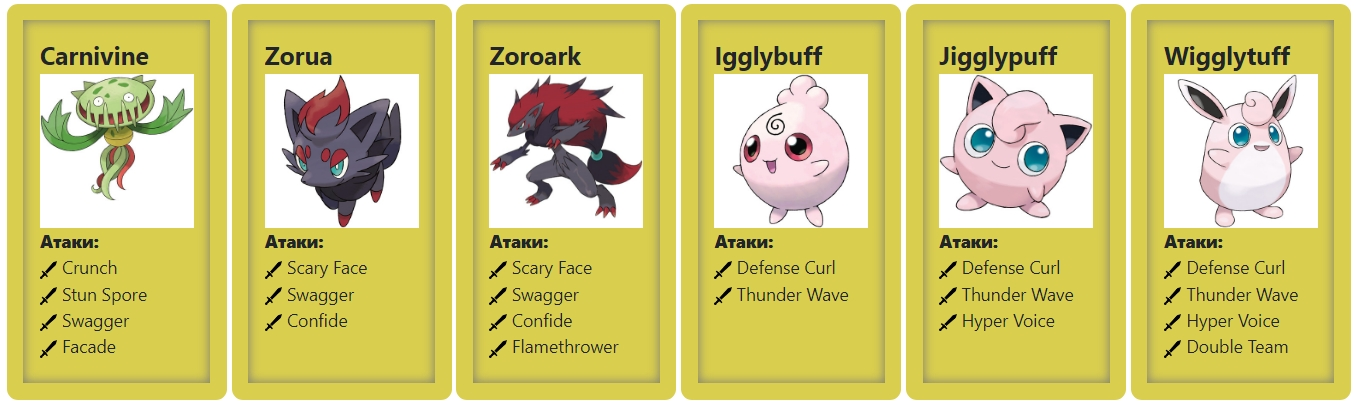
\includegraphics[width=\textwidth]{res/pokemons.jpeg}
        % }} % ограничение области действия параметров
        \caption{Покемоны и их атаки}
        \label{fig:enter-label}
    \end{figure}

%    \begin{center}
%        ' ' '
%    \end{center}

    \newpage
    \Section{Выполнение задания.}
    Задание было выполнено в редакторе кода IntejjiJ IDEA, собрано в \verb|jar| файл \verb|lab2.jar| и загружено в Git репозиторий на GitHub.
%    \newpage
    \Subsection{Листинги кода}
    Листинг из файла~\ref{lst:java}
    \lstinputlisting[caption={Исходный код главного класса программы},label={lst:java},language=Java]{../src/Main.java}

%    Листинг в код latex \ref{lst:sql}
%    \begin{lstlisting}[caption={SQL},label={lst:sql}]
%declare @t table(
%  id int
%)
%    \end{lstlisting}

%    Листинг прямо в текст: \lstinline[columns=fixed]{declare}. Либо еще так: \verb|declare|.

%    Вставленное изображение с описанием и шириной по тексту.
    \begin{figure}[H] % 'H' -- вставить тут же (подключен модуль), обычный вариант: 'htpb'
        \centering
        % { граница для иллюстрации
        % \setlength{\fboxsep}{0pt}% убрать отсутп от границы
        % \setlength{\fboxrule}{1pt}%
        % \fbox{%
        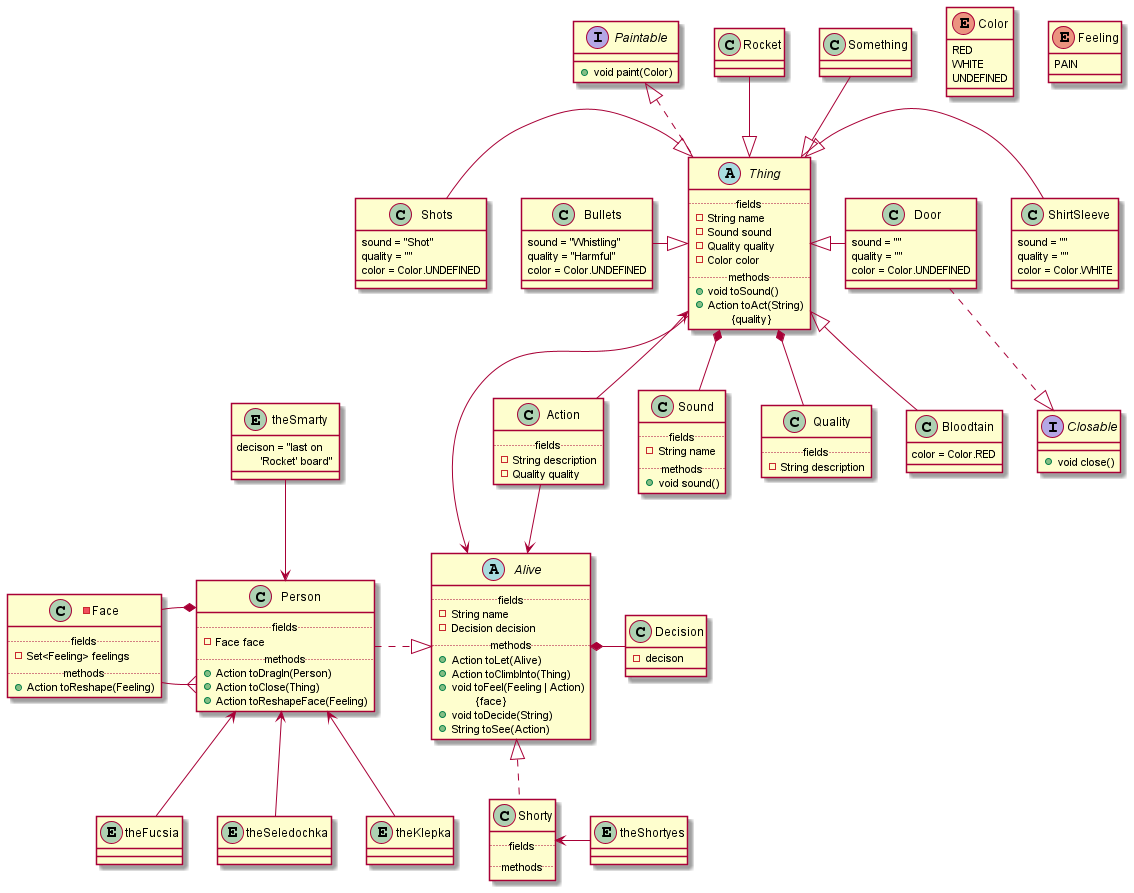
\includegraphics[width=\textwidth]{res/UML-class-diagram.png}
        % }} % ограничение области действия параметров
        \caption{UML диаграмма классов с методами и полями}
        \label{fig:enter-label2}
    \end{figure}


% Выполнение задания...
    \Section{Результат работы программы.}
%    \Subsection{Первый запуск.}
    \begin{lstlisting}[caption={Результат выполнения программы},label={lst:result}]
    Carnivine Carnivine from the team Red enters the battle!
    Igglybuff Iglybuff from the team Black enters the battle!
    Carnivine Carnivine is using Crunch. The user crunches up the target with sharp fangs. This may also lower the target’s Defense stat.
    Igglybuff Iglybuff loses 3 hit points.

    Igglybuff Iglybuff is using Thunder Wave. The user launches a weak jolt of electricity that paralyzes the target.
    Carnivine Carnivine is paralyzed

    Igglybuff Iglybuff is using Thunder Wave. The user launches a weak jolt of electricity that paralyzes the target.


    Igglybuff Iglybuff is using Thunder Wave. The user launches a weak jolt of electricity that paralyzes the target.


    Carnivine Carnivine is using Stun Spore. The user scatters a cloud of numbing powder that paralyzes the target.
    Igglybuff Iglybuff is paralyzed

    Igglybuff Iglybuff misses

    Igglybuff Iglybuff misses


    Carnivine Carnivine is using Stun Spore. The user scatters a cloud of numbing powder that paralyzes the target.


    Igglybuff Iglybuff is using Thunder Wave. The user launches a weak jolt of electricity that paralyzes the target.

    Igglybuff Iglybuff is using Thunder Wave. The user launches a weak jolt of electricity that paralyzes the target.

    Carnivine Carnivine is using Stun Spore. The user scatters a cloud of numbing powder that paralyzes the target.

    Igglybuff Iglybuff is using Thunder Wave. The user launches a weak jolt of electricity that paralyzes the target.

    Carnivine Carnivine is using Stun Spore. The user scatters a cloud of numbing powder that paralyzes the target.


    Igglybuff Iglybuff misses


    Igglybuff Iglybuff misses

    Igglybuff Iglybuff misses

    Carnivine Carnivine is using Stun Spore. The user scatters a cloud of numbing powder that paralyzes the target.

    Igglybuff Iglybuff misses

    Carnivine Carnivine is using Crunch. The user crunches up the target with sharp fangs. This may also lower the target’s Defense stat.
    Critical hit!
    Carnivine Carnivine loses 9 hit points.

    Carnivine Carnivine is using Crunch. The user crunches up the target with sharp fangs. This may also lower the target’s Defense stat.
    Critical hit!
    Carnivine Carnivine loses 7 hit points.
    Both pokemons faint.
    Zorua Zorua from the team Red enters the battle!
    Zorua Zorua is using Scary Face. The user frightens the target with a scary face to harshly lower its Speed stat.
    Igglybuff Iglybuff decreases speed.


    Zorua Zorua misses

    Igglybuff Iglybuff misses

    Zorua Zorua is using Scary Face. The user frightens the target with a scary face to harshly lower its Speed stat.
    Igglybuff Iglybuff decreases speed.


    Zorua Zorua is using Swagger. The user enrages and confuses the target. However, this also sharply boosts the target’s Attack stat.
    Igglybuff Iglybuff increases attack.


    Zorua Zorua misses

    Igglybuff Iglybuff hits himself in confusion.
    Igglybuff Iglybuff loses 5 hit points.

    Zorua Zorua misses

    Igglybuff Iglybuff misses

    Zorua Zorua misses

    Igglybuff Iglybuff is using Thunder Wave. The user launches a weak jolt of electricity that paralyzes the target.
    Zorua Zorua is paralyzed

    Zorua Zorua misses

    Igglybuff Iglybuff hits himself in confusion.
    Igglybuff Iglybuff loses 4 hit points.



    Zorua Zorua is using Scary Face. The user frightens the target with a scary face to harshly lower its Speed stat.
    Igglybuff Iglybuff decreases speed.


    Zorua Zorua misses


    Zorua Zorua is using Scary Face. The user frightens the target with a scary face to harshly lower its Speed stat.
    Igglybuff Iglybuff decreases speed.


    Zorua Zorua is using Swagger. The user enrages and confuses the target. However, this also sharply boosts the target’s Attack stat.
    Igglybuff Iglybuff increases attack.


    Zorua Zorua misses

    Igglybuff Iglybuff hits himself in confusion.
    Igglybuff Iglybuff loses 4 hit points.
    Igglybuff Iglybuff faints.
    Jigglypuff Jigglypuff from the team Black enters the battle!
    Zorua Zorua misses

    Jigglypuff Jigglypuff is using Thunder Wave. The user launches a weak jolt of electricity that paralyzes the target.

    Zorua Zorua misses

    Jigglypuff Jigglypuff is using Hyper Voice. The user attacks by letting loose a horribly loud, resounding cry.
    Zorua Zorua loses 10 hit points.

    Zorua Zorua is using Scary Face. The user frightens the target with a scary face to harshly lower its Speed stat.
    Jigglypuff Jigglypuff decreases speed.

    Jigglypuff Jigglypuff is using Thunder Wave. The user launches a weak jolt of electricity that paralyzes the target.

    Zorua Zorua is using Swagger. The user enrages and confuses the target. However, this also sharply boosts the target’s Attack stat.
    Zorua Zorua increases attack.

    Zorua Zorua is using Swagger. The user enrages and confuses the target. However, this also sharply boosts the target’s Attack stat.
    Zorua Zorua increases attack.

    Jigglypuff Jigglypuff is using Hyper Voice. The user attacks by letting loose a horribly loud, resounding cry.
    Critical hit!
    Jigglypuff Jigglypuff loses 16 hit points.
    Both pokemons faint.
    Wigglytuff Wigglytuff from the team Black enters the battle!
    Zorua Zorua is using Scary Face. The user frightens the target with a scary face to harshly lower its Speed stat.
    Wigglytuff Wigglytuff decreases speed.

    Wigglytuff Wigglytuff is using Thunder Wave. The user launches a weak jolt of electricity that paralyzes the target.

    Zorua Zorua is using Scary Face. The user frightens the target with a scary face to harshly lower its Speed stat.
    Zorua Zorua decreases speed.

    Zorua Zorua is using Scary Face. The user frightens the target with a scary face to harshly lower its Speed stat.
    Zorua Zorua decreases speed.

    Wigglytuff Wigglytuff misses

    Zorua Zorua hits himself in confusion.
    Zorua Zorua loses 3 hit points.
    Zorua Zorua faints.
    Zoroark Zoroark from the team Red enters the battle!
    Wigglytuff Wigglytuff misses

    Zoroark Zoroark is using Swagger. The user enrages and confuses the target. However, this also sharply boosts the target’s Attack stat.
    Wigglytuff Wigglytuff increases attack.

    Wigglytuff Wigglytuff is using Hyper Voice. The user attacks by letting loose a horribly loud, resounding cry.
    Critical hit!
    Zoroark Zoroark loses 13 hit points.
    Zoroark Zoroark faints.
    Team Red loses its last Pokemon.
    The team Black wins the battle!
    \end{lstlisting}

    \Section{Вывод}
% Вывод...
    Во время выполнения лабораторной работы я изучил принципы ООП, научился импортировать \verb|jar| файлы как библиотеки, научился расширять классы и рабоать с модификаторами доступа, ознакомился с системой сборки \verb|Gradle|, \verb|IDEA|. Также в процессе выполения я тесно работал с документацией\cite{sedoc} на библиотеку для покемонов и сторонними сайтами для поиска информации о покемонах (PokemonDB\cite{pokemondb}). Полученные мною знания являются необходимой базой для дальнейшего изучения языка и разработки уже более комлпексных проектов.\\
    Помимо этого, я ознакомился с способами создания UML диаграм и сделал диаграмму на практике при помощи встроенных в IDE средств.
% -- из biblist
    \newpage
%<<<<<<<<<<<<<<<<<<<<<< КОД РАБОТЫ <<<<<<<<<<<<<<<<<<<<<<<<


%>>>>>>>>>>>>>>>> СПИСОК ЛИТЕРАТУРЫ >>>>>>>>>>>>>>>>>>>>>>>
    \begin{thebibliography}{}
    \bibitem{github} Cсылка на личный репозиторий GitHub: \url{https://github.com/pozitp/itmo-labs/tree/main/opd/lab1}\\
    \bibitem{gnudoc} Ссылка на официальную документацию GNU по coreutils (базовые команды *NIX): \url{https://www.gnu.org/software/coreutils/manual/coreutils.html}\\
    \bibitem{gitdoc} Ссылка на официальную документацию Git с базовыми командами для работы с системами конторя версий файлов: \url{https://git-scm.com/docs/giteveryday}\\
    \bibitem{archwiki} Ссылка на ArchWiki: \url{https://wiki.archlinux.org}\\
    \bibitem{gentoowiki} Ссылка на Gentoo Wiki: \url{https://wiki.gentoo.org}\\

\end{thebibliography}  % Для соответсвия гост, придется доработать. Нужен файл .bib
%<<<<<<<<<<<<<<<<<<<< СПИСОК ЛИТЕРАТУРЫ <<<<<<<<<<<<<<<<<<<


\end{document}
%<<<<<<<<<<<<<<<< ,,,,,,,,,,,,,,,,,,,,,,, <<<<<<<<<<<<<<<<<
%<<<<<<<<<<<<<<<<<<< СОДЕРЖИМОЕ ОТЧЕТА <<<<<<<<<<<<<<<<<<<<
